% !TeX root = diploma.tex

\begin{figure}[p]\label{fig:1}
\centering
\subfloat[а)]{
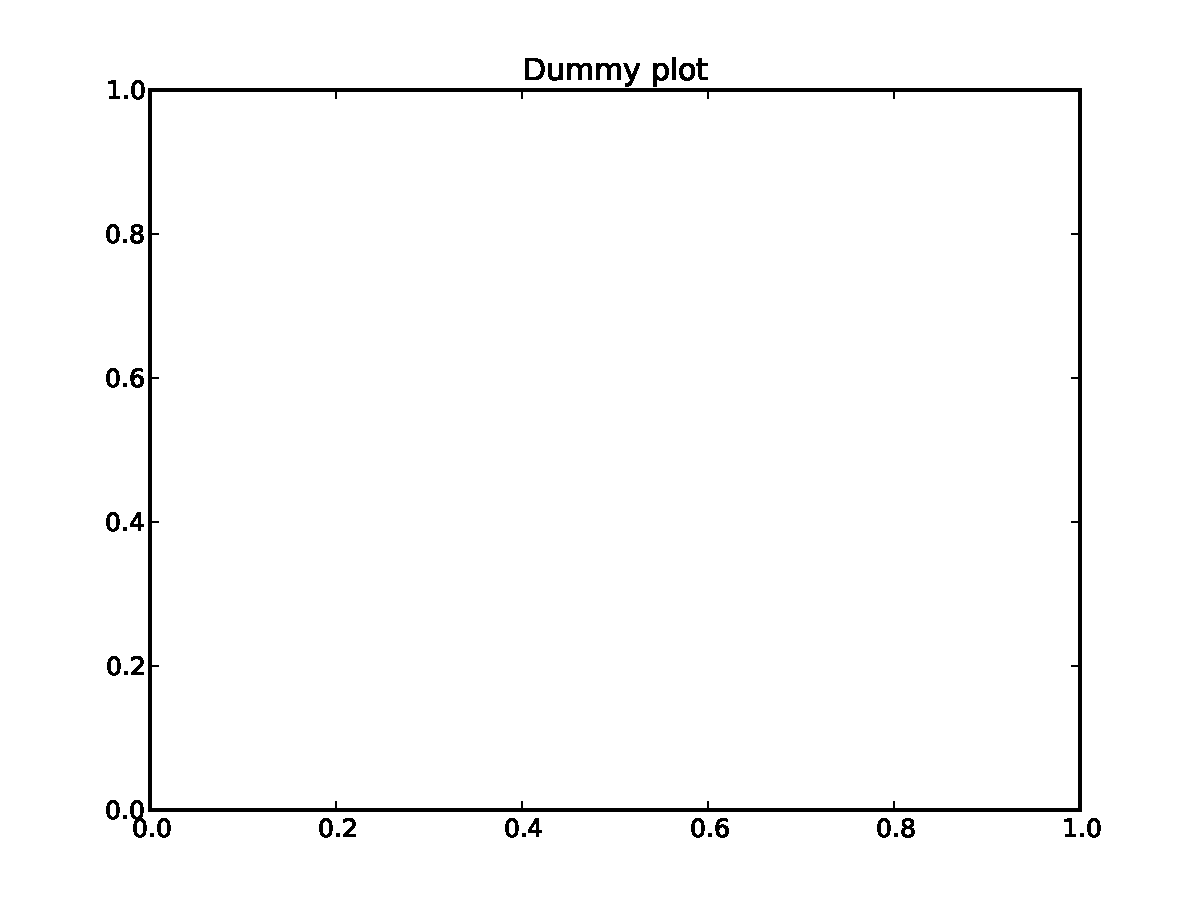
\includegraphics[width = 0.5\textwidth]{figs/dummy.pdf}
\label{fig:dpinitk}}
\subfloat[б)]{
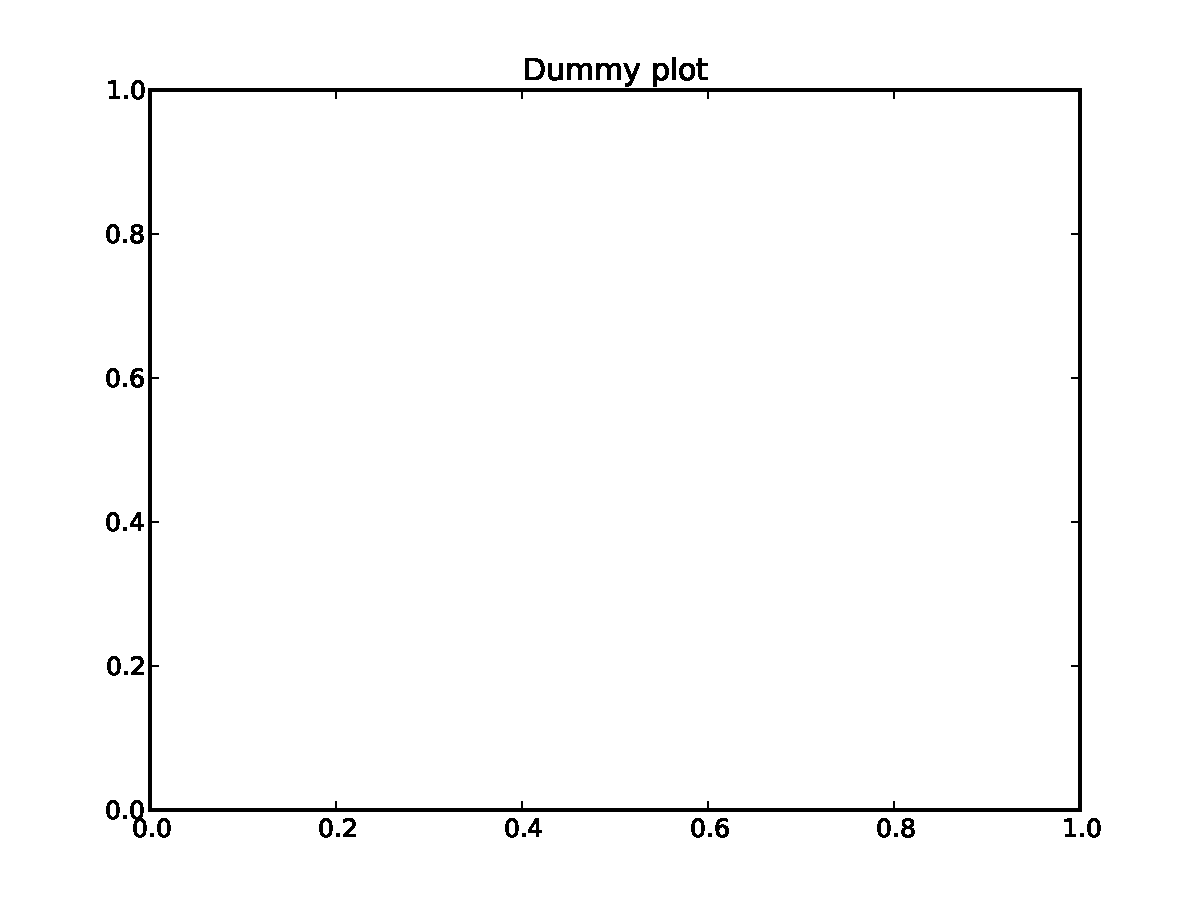
\includegraphics[width = 0.5\textwidth]{figs/dummy.pdf}
\label{fig:gpinita}}
\newline
\subfloat[в)]{
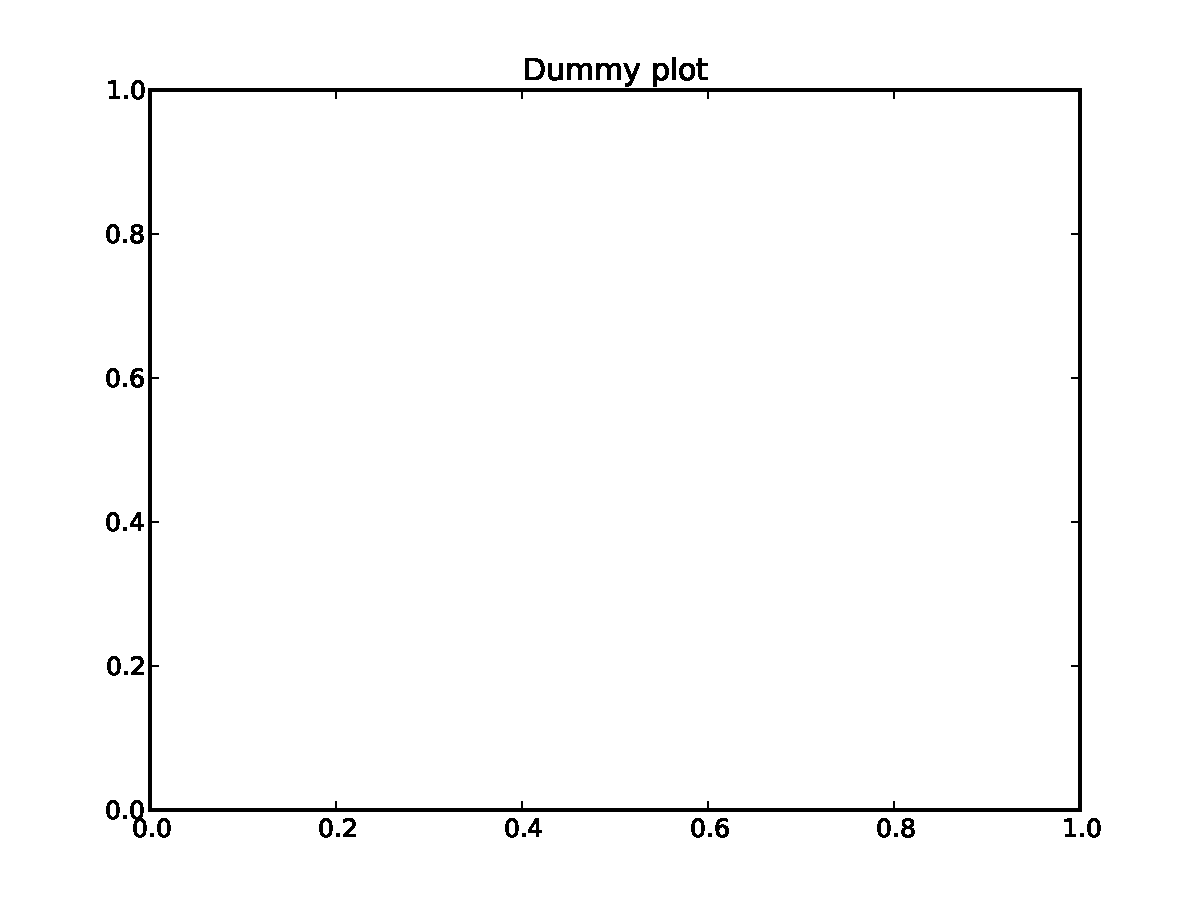
\includegraphics[width = 0.5\textwidth]{figs/dummy.pdf}
\label{fig:gpinitcpt}}
\newline
\caption{Результаты вычислений для $g= -1.241$, $p_{icp}= -0.088$, $p_{cp}=-0.137$:
\newlineа) для волнового числа; 
\newlineб) для амплитуды ПП;
\newlineв) для скачка теплоемкости, отнесенного к температуре.}
\end{figure}